\documentclass[twoside]{book}

% Packages required by doxygen
\usepackage{fixltx2e}
\usepackage{calc}
\usepackage{doxygen}
\usepackage[export]{adjustbox} % also loads graphicx
\usepackage{graphicx}
\usepackage[utf8]{inputenc}
\usepackage{makeidx}
\usepackage{multicol}
\usepackage{multirow}
\PassOptionsToPackage{warn}{textcomp}
\usepackage{textcomp}
\usepackage[nointegrals]{wasysym}
\usepackage[table]{xcolor}

% Font selection
\usepackage[T1]{fontenc}
\usepackage[scaled=.90]{helvet}
\usepackage{courier}
\usepackage{amssymb}
\usepackage{sectsty}
\renewcommand{\familydefault}{\sfdefault}
\allsectionsfont{%
  \fontseries{bc}\selectfont%
  \color{darkgray}%
}
\renewcommand{\DoxyLabelFont}{%
  \fontseries{bc}\selectfont%
  \color{darkgray}%
}
\newcommand{\+}{\discretionary{\mbox{\scriptsize$\hookleftarrow$}}{}{}}

% Page & text layout
\usepackage{geometry}
\geometry{%
  a4paper,%
  top=2.5cm,%
  bottom=2.5cm,%
  left=2.5cm,%
  right=2.5cm%
}
\tolerance=750
\hfuzz=15pt
\hbadness=750
\setlength{\emergencystretch}{15pt}
\setlength{\parindent}{0cm}
\setlength{\parskip}{3ex plus 2ex minus 2ex}
\makeatletter
\renewcommand{\paragraph}{%
  \@startsection{paragraph}{4}{0ex}{-1.0ex}{1.0ex}{%
    \normalfont\normalsize\bfseries\SS@parafont%
  }%
}
\renewcommand{\subparagraph}{%
  \@startsection{subparagraph}{5}{0ex}{-1.0ex}{1.0ex}{%
    \normalfont\normalsize\bfseries\SS@subparafont%
  }%
}
\makeatother

% Headers & footers
\usepackage{fancyhdr}
\pagestyle{fancyplain}
\fancyhead[LE]{\fancyplain{}{\bfseries\thepage}}
\fancyhead[CE]{\fancyplain{}{}}
\fancyhead[RE]{\fancyplain{}{\bfseries\leftmark}}
\fancyhead[LO]{\fancyplain{}{\bfseries\rightmark}}
\fancyhead[CO]{\fancyplain{}{}}
\fancyhead[RO]{\fancyplain{}{\bfseries\thepage}}
\fancyfoot[LE]{\fancyplain{}{}}
\fancyfoot[CE]{\fancyplain{}{}}
\fancyfoot[RE]{\fancyplain{}{\bfseries\scriptsize Generated by Doxygen }}
\fancyfoot[LO]{\fancyplain{}{\bfseries\scriptsize Generated by Doxygen }}
\fancyfoot[CO]{\fancyplain{}{}}
\fancyfoot[RO]{\fancyplain{}{}}
\renewcommand{\footrulewidth}{0.4pt}
\renewcommand{\chaptermark}[1]{%
  \markboth{#1}{}%
}
\renewcommand{\sectionmark}[1]{%
  \markright{\thesection\ #1}%
}

% Indices & bibliography
\usepackage{natbib}
\usepackage[titles]{tocloft}
\setcounter{tocdepth}{3}
\setcounter{secnumdepth}{5}
\makeindex

% Hyperlinks (required, but should be loaded last)
\usepackage{ifpdf}
\ifpdf
  \usepackage[pdftex,pagebackref=true]{hyperref}
\else
  \usepackage[ps2pdf,pagebackref=true]{hyperref}
\fi
\hypersetup{%
  colorlinks=true,%
  linkcolor=blue,%
  citecolor=blue,%
  unicode%
}

% Custom commands
\newcommand{\clearemptydoublepage}{%
  \newpage{\pagestyle{empty}\cleardoublepage}%
}

\usepackage{caption}
\captionsetup{labelsep=space,justification=centering,font={bf},singlelinecheck=off,skip=4pt,position=top}

%===== C O N T E N T S =====

\begin{document}

% Titlepage & ToC
\hypersetup{pageanchor=false,
             bookmarksnumbered=true,
             pdfencoding=unicode
            }
\pagenumbering{alph}
\begin{titlepage}
\vspace*{7cm}
\begin{center}%
{\Large The Locomotion Package }\\
\vspace*{1cm}
{\large Generated by Doxygen 1.8.13}\\
\end{center}
\end{titlepage}
\clearemptydoublepage
\pagenumbering{roman}
\tableofcontents
\clearemptydoublepage
\pagenumbering{arabic}
\hypersetup{pageanchor=true}

%--- Begin generated contents ---
\chapter{Hierarchical Index}
\section{Class Hierarchy}
This inheritance list is sorted roughly, but not completely, alphabetically\+:\begin{DoxyCompactList}
\item \contentsline{section}{service\+\_\+node.\+Dijkstra}{\pageref{classservice__node_1_1Dijkstra}}{}
\begin{DoxyCompactList}
\item \contentsline{section}{service\+\_\+node.\+Graph\+\_\+d}{\pageref{classservice__node_1_1Graph__d}}{}
\end{DoxyCompactList}
\item \contentsline{section}{service\+\_\+node.\+Map}{\pageref{classservice__node_1_1Map}}{}
\item \contentsline{section}{service\+\_\+node.\+Math\+Operations}{\pageref{classservice__node_1_1MathOperations}}{}
\item \contentsline{section}{service\+\_\+node.\+Obstacles}{\pageref{classservice__node_1_1Obstacles}}{}
\item \contentsline{section}{service\+\_\+node.\+Path}{\pageref{classservice__node_1_1Path}}{}
\item \contentsline{section}{service\+\_\+node.\+Points}{\pageref{classservice__node_1_1Points}}{}
\item \contentsline{section}{service\+\_\+node.\+Ways}{\pageref{classservice__node_1_1Ways}}{}
\end{DoxyCompactList}

\chapter{Class Index}
\section{Class List}
Here are the classes, structs, unions and interfaces with brief descriptions\+:\begin{DoxyCompactList}
\item\contentsline{section}{\hyperlink{classservice__node_1_1Dijkstra}{service\+\_\+node.\+Dijkstra} }{\pageref{classservice__node_1_1Dijkstra}}{}
\item\contentsline{section}{\hyperlink{classservice__node_1_1Graph__d}{service\+\_\+node.\+Graph\+\_\+d} }{\pageref{classservice__node_1_1Graph__d}}{}
\item\contentsline{section}{\hyperlink{classMapDesign_1_1Map}{Map\+Design.\+Map} }{\pageref{classMapDesign_1_1Map}}{}
\item\contentsline{section}{\hyperlink{classMapDesign_1_1MathOperations}{Map\+Design.\+Math\+Operations} }{\pageref{classMapDesign_1_1MathOperations}}{}
\item\contentsline{section}{\hyperlink{classservice__node_1_1MathOperations}{service\+\_\+node.\+Math\+Operations} }{\pageref{classservice__node_1_1MathOperations}}{}
\item\contentsline{section}{\hyperlink{classMapDesign_1_1Obstacles}{Map\+Design.\+Obstacles} }{\pageref{classMapDesign_1_1Obstacles}}{}
\item\contentsline{section}{\hyperlink{classservice__node_1_1Path}{service\+\_\+node.\+Path} }{\pageref{classservice__node_1_1Path}}{}
\item\contentsline{section}{\hyperlink{classMapDesign_1_1Points}{Map\+Design.\+Points} }{\pageref{classMapDesign_1_1Points}}{}
\item\contentsline{section}{\hyperlink{classservice__node_1_1Points}{service\+\_\+node.\+Points} }{\pageref{classservice__node_1_1Points}}{}
\item\contentsline{section}{\hyperlink{classMapDesign_1_1Ways}{Map\+Design.\+Ways} }{\pageref{classMapDesign_1_1Ways}}{}
\end{DoxyCompactList}

\chapter{Class Documentation}
\hypertarget{classservice__node_1_1Dijkstra}{}\section{service\+\_\+node.\+Dijkstra Class Reference}
\label{classservice__node_1_1Dijkstra}\index{service\+\_\+node.\+Dijkstra@{service\+\_\+node.\+Dijkstra}}


Inheritance diagram for service\+\_\+node.\+Dijkstra\+:
\nopagebreak
\begin{figure}[H]
\begin{center}
\leavevmode
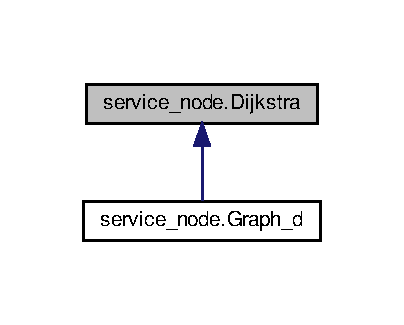
\includegraphics[width=194pt]{classservice__node_1_1Dijkstra__inherit__graph}
\end{center}
\end{figure}
\subsection*{Public Member Functions}
\begin{DoxyCompactItemize}
\item 
\mbox{\Hypertarget{classservice__node_1_1Dijkstra_a6d1a519973491eca0cdd433a8140035d}\label{classservice__node_1_1Dijkstra_a6d1a519973491eca0cdd433a8140035d}} 
def {\bfseries Calculate\+Path} (self, graph, initial, end)
\end{DoxyCompactItemize}


The documentation for this class was generated from the following file\+:\begin{DoxyCompactItemize}
\item 
/home/adnanhd/\+Examples/\+Rover/catkin\+\_\+ws/src/leo-\/rover-\/locomotion/nodes/service\+\_\+node.\+py\end{DoxyCompactItemize}

\hypertarget{classservice__node_1_1Graph__d}{}\section{service\+\_\+node.\+Graph\+\_\+d Class Reference}
\label{classservice__node_1_1Graph__d}\index{service\+\_\+node.\+Graph\+\_\+d@{service\+\_\+node.\+Graph\+\_\+d}}


Inheritance diagram for service\+\_\+node.\+Graph\+\_\+d\+:\nopagebreak
\begin{figure}[H]
\begin{center}
\leavevmode
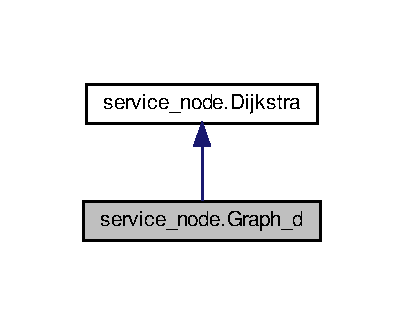
\includegraphics[width=194pt]{classservice__node_1_1Graph__d__inherit__graph}
\end{center}
\end{figure}


Collaboration diagram for service\+\_\+node.\+Graph\+\_\+d\+:\nopagebreak
\begin{figure}[H]
\begin{center}
\leavevmode
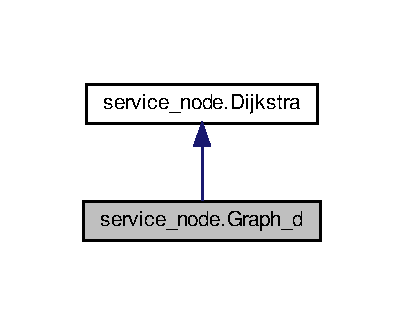
\includegraphics[width=194pt]{classservice__node_1_1Graph__d__coll__graph}
\end{center}
\end{figure}
\subsection*{Public Member Functions}
\begin{DoxyCompactItemize}
\item 
def \hyperlink{classservice__node_1_1Graph__d_a76ed82f1e5e08fb2fbd979a1c7a988ee}{\+\_\+\+\_\+init\+\_\+\+\_\+} (self)
\item 
\mbox{\Hypertarget{classservice__node_1_1Graph__d_adaf7f491fe653300d1ccfac05ee36eff}\label{classservice__node_1_1Graph__d_adaf7f491fe653300d1ccfac05ee36eff}} 
def {\bfseries Add\+Edges} (self, from\+\_\+node, to\+\_\+node, roguhness)
\end{DoxyCompactItemize}
\subsection*{Public Attributes}
\begin{DoxyCompactItemize}
\item 
\mbox{\Hypertarget{classservice__node_1_1Graph__d_ac8312e991685daf3d8ae7f1c89734287}\label{classservice__node_1_1Graph__d_ac8312e991685daf3d8ae7f1c89734287}} 
{\bfseries Possible\+Path\+Points}
\item 
\mbox{\Hypertarget{classservice__node_1_1Graph__d_a7a94a0789e58110d2e5fece70623f53c}\label{classservice__node_1_1Graph__d_a7a94a0789e58110d2e5fece70623f53c}} 
{\bfseries Point\+Roughnesseses}
\end{DoxyCompactItemize}


\subsection{Constructor \& Destructor Documentation}
\mbox{\Hypertarget{classservice__node_1_1Graph__d_a76ed82f1e5e08fb2fbd979a1c7a988ee}\label{classservice__node_1_1Graph__d_a76ed82f1e5e08fb2fbd979a1c7a988ee}} 
\index{service\+\_\+node\+::\+Graph\+\_\+d@{service\+\_\+node\+::\+Graph\+\_\+d}!\+\_\+\+\_\+init\+\_\+\+\_\+@{\+\_\+\+\_\+init\+\_\+\+\_\+}}
\index{\+\_\+\+\_\+init\+\_\+\+\_\+@{\+\_\+\+\_\+init\+\_\+\+\_\+}!service\+\_\+node\+::\+Graph\+\_\+d@{service\+\_\+node\+::\+Graph\+\_\+d}}
\subsubsection{\texorpdfstring{\+\_\+\+\_\+init\+\_\+\+\_\+()}{\_\_init\_\_()}}
{\footnotesize\ttfamily def service\+\_\+node.\+Graph\+\_\+d.\+\_\+\+\_\+init\+\_\+\+\_\+ (\begin{DoxyParamCaption}\item[{}]{self }\end{DoxyParamCaption})}

\begin{DoxyVerb}self.edges is a dict of all possible next nodes
e.g. {'X': ['A', 'B', 'C', 'E'], ...}
self.roughnesss has all the roughnesss between two nodes,
with the two nodes as a tuple as the key
e.g. {('X', 'A'): 7, ('X', 'B'): 2, ...}
\end{DoxyVerb}
 

The documentation for this class was generated from the following file\+:\begin{DoxyCompactItemize}
\item 
/home/adnanhd/\+Examples/\+Rover/catkin\+\_\+ws/src/leo\+\_\+rover\+\_\+localization/nodes/service\+\_\+node.\+py\end{DoxyCompactItemize}

\hypertarget{classMapDesign_1_1Map}{}\section{Map\+Design.\+Map Class Reference}
\label{classMapDesign_1_1Map}\index{Map\+Design.\+Map@{Map\+Design.\+Map}}
\subsection*{Public Member Functions}
\begin{DoxyCompactItemize}
\item 
\mbox{\Hypertarget{classMapDesign_1_1Map_a4857633ee3e8709f1b2712f06f244b93}\label{classMapDesign_1_1Map_a4857633ee3e8709f1b2712f06f244b93}} 
def {\bfseries \+\_\+\+\_\+init\+\_\+\+\_\+} (self, mapsize=tuple, screensize=tuple)
\item 
\mbox{\Hypertarget{classMapDesign_1_1Map_ac46bd07ecbf51504b15153782e79c829}\label{classMapDesign_1_1Map_ac46bd07ecbf51504b15153782e79c829}} 
def {\bfseries find\+Map\+Size} (self, mapsize, screensize)
\end{DoxyCompactItemize}
\subsection*{Public Attributes}
\begin{DoxyCompactItemize}
\item 
\mbox{\Hypertarget{classMapDesign_1_1Map_a677032aa422a2151a2e8a3a3eb57eb25}\label{classMapDesign_1_1Map_a677032aa422a2151a2e8a3a3eb57eb25}} 
{\bfseries imagesize}
\item 
\mbox{\Hypertarget{classMapDesign_1_1Map_a322565c2c24bb43f8f945d0ee3f06e2a}\label{classMapDesign_1_1Map_a322565c2c24bb43f8f945d0ee3f06e2a}} 
{\bfseries pixelsize}
\end{DoxyCompactItemize}


The documentation for this class was generated from the following file\+:\begin{DoxyCompactItemize}
\item 
/home/adnanhd/\+Examples/\+Rover/catkin\+\_\+ws/src/leo\+\_\+rover\+\_\+localization/nodes/Map\+Design.\+py\end{DoxyCompactItemize}

\hypertarget{classMapDesign_1_1MathOperations}{}\section{Map\+Design.\+Math\+Operations Class Reference}
\label{classMapDesign_1_1MathOperations}\index{Map\+Design.\+Math\+Operations@{Map\+Design.\+Math\+Operations}}
\subsection*{Public Member Functions}
\begin{DoxyCompactItemize}
\item 
\mbox{\Hypertarget{classMapDesign_1_1MathOperations_a17956efa84f9873b11a8ec0a45b46929}\label{classMapDesign_1_1MathOperations_a17956efa84f9873b11a8ec0a45b46929}} 
def {\bfseries lenght\+Of\+Lines} (self, Coords=\mbox{[}$\,$\mbox{]}, roughness=\char`\"{}Infinity\char`\"{})
\item 
\mbox{\Hypertarget{classMapDesign_1_1MathOperations_acf2148fd6440dbefab6fb5f8ed4d96eb}\label{classMapDesign_1_1MathOperations_acf2148fd6440dbefab6fb5f8ed4d96eb}} 
def {\bfseries does\+Collide} (self, Pairs=\mbox{[}()\mbox{]}, Edges=\mbox{[}()\mbox{]})
\item 
\mbox{\Hypertarget{classMapDesign_1_1MathOperations_a764a8e6e93168ed3eb288fafb64e2ab5}\label{classMapDesign_1_1MathOperations_a764a8e6e93168ed3eb288fafb64e2ab5}} 
def {\bfseries functions\+Of\+Edges} (self, Edges=\mbox{[}$\,$\mbox{]})
\end{DoxyCompactItemize}


The documentation for this class was generated from the following file\+:\begin{DoxyCompactItemize}
\item 
/home/adnanhd/\+Examples/\+Rover/catkin\+\_\+ws/src/leo\+\_\+rover\+\_\+localization/nodes/Map\+Design.\+py\end{DoxyCompactItemize}

\hypertarget{classservice__node_1_1MathOperations}{}\section{service\+\_\+node.\+Math\+Operations Class Reference}
\label{classservice__node_1_1MathOperations}\index{service\+\_\+node.\+Math\+Operations@{service\+\_\+node.\+Math\+Operations}}
\subsection*{Public Member Functions}
\begin{DoxyCompactItemize}
\item 
\mbox{\Hypertarget{classservice__node_1_1MathOperations_af40dad96f5992cbd8ea64793050ca100}\label{classservice__node_1_1MathOperations_af40dad96f5992cbd8ea64793050ca100}} 
def {\bfseries lenght\+Of\+Lines} (self, Coords=\mbox{[}$\,$\mbox{]}, roughness=\char`\"{}Infinity\char`\"{})
\item 
\mbox{\Hypertarget{classservice__node_1_1MathOperations_a44c83fcab4c8fbed72c5b4a284441c7e}\label{classservice__node_1_1MathOperations_a44c83fcab4c8fbed72c5b4a284441c7e}} 
def {\bfseries does\+Collide} (self, Pairs=\mbox{[}()\mbox{]}, Edges=\mbox{[}()\mbox{]})
\item 
\mbox{\Hypertarget{classservice__node_1_1MathOperations_ace96f7bbddc5b3f76973f7cfc792e043}\label{classservice__node_1_1MathOperations_ace96f7bbddc5b3f76973f7cfc792e043}} 
def {\bfseries functions\+Of\+Edges} (self, Edges=\mbox{[}$\,$\mbox{]})
\end{DoxyCompactItemize}


The documentation for this class was generated from the following file\+:\begin{DoxyCompactItemize}
\item 
/home/adnanhd/\+Examples/\+Rover/catkin\+\_\+ws/src/leo-\/rover-\/locomotion/nodes/service\+\_\+node.\+py\end{DoxyCompactItemize}

\hypertarget{classMapDesign_1_1Obstacles}{}\section{Map\+Design.\+Obstacles Class Reference}
\label{classMapDesign_1_1Obstacles}\index{Map\+Design.\+Obstacles@{Map\+Design.\+Obstacles}}
\subsection*{Public Member Functions}
\begin{DoxyCompactItemize}
\item 
\mbox{\Hypertarget{classMapDesign_1_1Obstacles_ab1be7e3b82bf7af51c2dfb069f33c824}\label{classMapDesign_1_1Obstacles_ab1be7e3b82bf7af51c2dfb069f33c824}} 
def {\bfseries \+\_\+\+\_\+init\+\_\+\+\_\+} (self, Coords, Roughness=\char`\"{}Infinity\char`\"{})
\item 
\mbox{\Hypertarget{classMapDesign_1_1Obstacles_a7d48983e63e4ac175438d21b5e5df722}\label{classMapDesign_1_1Obstacles_a7d48983e63e4ac175438d21b5e5df722}} 
def {\bfseries Coords\+To\+Edges} (self)
\item 
\mbox{\Hypertarget{classMapDesign_1_1Obstacles_a62327f4b65d7a5c20b509862ceedd92a}\label{classMapDesign_1_1Obstacles_a62327f4b65d7a5c20b509862ceedd92a}} 
def {\bfseries Shift\+Coords} (self, number=1)
\end{DoxyCompactItemize}
\subsection*{Public Attributes}
\begin{DoxyCompactItemize}
\item 
\mbox{\Hypertarget{classMapDesign_1_1Obstacles_a7818fce9ea6250a9f319ef99019398cd}\label{classMapDesign_1_1Obstacles_a7818fce9ea6250a9f319ef99019398cd}} 
{\bfseries Coords}
\item 
\mbox{\Hypertarget{classMapDesign_1_1Obstacles_aa256d89ec86193cd6257ac407128f130}\label{classMapDesign_1_1Obstacles_aa256d89ec86193cd6257ac407128f130}} 
{\bfseries Inside\+Coords}
\item 
\mbox{\Hypertarget{classMapDesign_1_1Obstacles_a9ac9628450b43fe32fb70e53590fa160}\label{classMapDesign_1_1Obstacles_a9ac9628450b43fe32fb70e53590fa160}} 
{\bfseries Edges}
\item 
\mbox{\Hypertarget{classMapDesign_1_1Obstacles_a10a6682f8b5a18bfe96e4197812b7af4}\label{classMapDesign_1_1Obstacles_a10a6682f8b5a18bfe96e4197812b7af4}} 
{\bfseries Roughness}
\item 
\mbox{\Hypertarget{classMapDesign_1_1Obstacles_a7e8c3de6188ba056265772663bfb7807}\label{classMapDesign_1_1Obstacles_a7e8c3de6188ba056265772663bfb7807}} 
{\bfseries Mean\+Point}
\end{DoxyCompactItemize}


The documentation for this class was generated from the following file\+:\begin{DoxyCompactItemize}
\item 
/home/adnanhd/\+Examples/\+Rover/catkin\+\_\+ws/src/leo\+\_\+rover\+\_\+localization/nodes/Map\+Design.\+py\end{DoxyCompactItemize}

\hypertarget{classservice__node_1_1Path}{}\section{service\+\_\+node.\+Path Class Reference}
\label{classservice__node_1_1Path}\index{service\+\_\+node.\+Path@{service\+\_\+node.\+Path}}
\subsection*{Public Member Functions}
\begin{DoxyCompactItemize}
\item 
\mbox{\Hypertarget{classservice__node_1_1Path_ac66df455e00a98279d5db61985b8b3ff}\label{classservice__node_1_1Path_ac66df455e00a98279d5db61985b8b3ff}} 
def {\bfseries \+\_\+\+\_\+init\+\_\+\+\_\+} (self, ways, waylist)
\item 
\mbox{\Hypertarget{classservice__node_1_1Path_a9947fd0a2a144ef57cd75ed3f68829e0}\label{classservice__node_1_1Path_a9947fd0a2a144ef57cd75ed3f68829e0}} 
def {\bfseries Create\+Path} (self, Start\+\_\+\+Point, End\+\_\+\+Points=list)
\item 
\mbox{\Hypertarget{classservice__node_1_1Path_a6c2a4122062c23d7789375230a01f2bd}\label{classservice__node_1_1Path_a6c2a4122062c23d7789375230a01f2bd}} 
def {\bfseries Dijkstras\+Algorithm} (self, Start\+\_\+\+Point, End\+\_\+\+Point, ways)
\item 
\mbox{\Hypertarget{classservice__node_1_1Path_a39a4cd3962fbe30c2c3d835d23b6eff9}\label{classservice__node_1_1Path_a39a4cd3962fbe30c2c3d835d23b6eff9}} 
def {\bfseries Check\+Obstacles} (self, startpoint, endpoint, ways)
\item 
\mbox{\Hypertarget{classservice__node_1_1Path_a8cf17afe9bdbb156da13e24707f3df38}\label{classservice__node_1_1Path_a8cf17afe9bdbb156da13e24707f3df38}} 
def {\bfseries find\+Roughness} (self, Map)
\end{DoxyCompactItemize}
\subsection*{Public Attributes}
\begin{DoxyCompactItemize}
\item 
\mbox{\Hypertarget{classservice__node_1_1Path_a9d0a619d0d0fd5f2167b5229cbf65818}\label{classservice__node_1_1Path_a9d0a619d0d0fd5f2167b5229cbf65818}} 
{\bfseries Ways}
\item 
\mbox{\Hypertarget{classservice__node_1_1Path_a78a66c2a039df6318fe31aa7da84754b}\label{classservice__node_1_1Path_a78a66c2a039df6318fe31aa7da84754b}} 
{\bfseries path}
\end{DoxyCompactItemize}


The documentation for this class was generated from the following file\+:\begin{DoxyCompactItemize}
\item 
/home/adnanhd/\+Examples/\+Rover/catkin\+\_\+ws/src/leo\+\_\+rover\+\_\+localization/nodes/service\+\_\+node.\+py\end{DoxyCompactItemize}

\hypertarget{classMapDesign_1_1Points}{}\section{Map\+Design.\+Points Class Reference}
\label{classMapDesign_1_1Points}\index{Map\+Design.\+Points@{Map\+Design.\+Points}}
\subsection*{Public Member Functions}
\begin{DoxyCompactItemize}
\item 
\mbox{\Hypertarget{classMapDesign_1_1Points_ab17adbaa191fa0dfba22f1162693760b}\label{classMapDesign_1_1Points_ab17adbaa191fa0dfba22f1162693760b}} 
def {\bfseries \+\_\+\+\_\+init\+\_\+\+\_\+} (self, coords, Way)
\item 
\mbox{\Hypertarget{classMapDesign_1_1Points_a4838d0768aa997c969734a67aee08fca}\label{classMapDesign_1_1Points_a4838d0768aa997c969734a67aee08fca}} 
def {\bfseries Is\+It\+Inside} (self, Given\+Obstacle\+List=\mbox{[}$\,$\mbox{]})
\item 
\mbox{\Hypertarget{classMapDesign_1_1Points_a7b4479a5847dca344ef902f56cad7831}\label{classMapDesign_1_1Points_a7b4479a5847dca344ef902f56cad7831}} 
def {\bfseries Add\+Points\+To\+Pair\+List} (self, Given\+Obstacle\+List=\mbox{[}$\,$\mbox{]})
\end{DoxyCompactItemize}
\subsection*{Public Attributes}
\begin{DoxyCompactItemize}
\item 
\mbox{\Hypertarget{classMapDesign_1_1Points_a494438ab13122e025d36bd22b16a5c70}\label{classMapDesign_1_1Points_a494438ab13122e025d36bd22b16a5c70}} 
{\bfseries Coord}
\item 
\mbox{\Hypertarget{classMapDesign_1_1Points_a01100dbd216dd459decabf9949aed8a1}\label{classMapDesign_1_1Points_a01100dbd216dd459decabf9949aed8a1}} 
{\bfseries Roughness}
\end{DoxyCompactItemize}


The documentation for this class was generated from the following file\+:\begin{DoxyCompactItemize}
\item 
/home/adnanhd/\+Examples/\+Rover/catkin\+\_\+ws/src/leo\+\_\+rover\+\_\+localization/nodes/Map\+Design.\+py\end{DoxyCompactItemize}

\hypertarget{classservice__node_1_1Points}{}\section{service\+\_\+node.\+Points Class Reference}
\label{classservice__node_1_1Points}\index{service\+\_\+node.\+Points@{service\+\_\+node.\+Points}}
\subsection*{Public Member Functions}
\begin{DoxyCompactItemize}
\item 
\mbox{\Hypertarget{classservice__node_1_1Points_a4b61c9c2f75645cdb97d02a47485848f}\label{classservice__node_1_1Points_a4b61c9c2f75645cdb97d02a47485848f}} 
def {\bfseries \+\_\+\+\_\+init\+\_\+\+\_\+} (self, coords, Way)
\item 
\mbox{\Hypertarget{classservice__node_1_1Points_af36e30c73ec133c560d11ae983338dbe}\label{classservice__node_1_1Points_af36e30c73ec133c560d11ae983338dbe}} 
def {\bfseries Is\+It\+Inside} (self, Given\+Obstacle\+List=\mbox{[}$\,$\mbox{]})
\item 
\mbox{\Hypertarget{classservice__node_1_1Points_a8522e492d24585f354b324b0af5281c5}\label{classservice__node_1_1Points_a8522e492d24585f354b324b0af5281c5}} 
def {\bfseries Add\+Points\+To\+Pair\+List} (self, Given\+Obstacle\+List=\mbox{[}$\,$\mbox{]})
\end{DoxyCompactItemize}
\subsection*{Public Attributes}
\begin{DoxyCompactItemize}
\item 
\mbox{\Hypertarget{classservice__node_1_1Points_a5ad9393800d33cfdb3b1be4b94818a9d}\label{classservice__node_1_1Points_a5ad9393800d33cfdb3b1be4b94818a9d}} 
{\bfseries Coord}
\item 
\mbox{\Hypertarget{classservice__node_1_1Points_a9b66d38fcaa6f50c86c72aa290cb731b}\label{classservice__node_1_1Points_a9b66d38fcaa6f50c86c72aa290cb731b}} 
{\bfseries Roughness}
\end{DoxyCompactItemize}


The documentation for this class was generated from the following file\+:\begin{DoxyCompactItemize}
\item 
/home/adnanhd/\+Examples/\+Rover/catkin\+\_\+ws/src/leo\+\_\+rover\+\_\+localization/nodes/service\+\_\+node.\+py\end{DoxyCompactItemize}

\hypertarget{classMapDesign_1_1Ways}{}\section{Map\+Design.\+Ways Class Reference}
\label{classMapDesign_1_1Ways}\index{Map\+Design.\+Ways@{Map\+Design.\+Ways}}
\subsection*{Public Member Functions}
\begin{DoxyCompactItemize}
\item 
\mbox{\Hypertarget{classMapDesign_1_1Ways_a09120cb730092d5026f372277c79cdf0}\label{classMapDesign_1_1Ways_a09120cb730092d5026f372277c79cdf0}} 
def {\bfseries \+\_\+\+\_\+init\+\_\+\+\_\+} (self, Obstacles\+List=\mbox{[}$\,$\mbox{]})
\item 
\mbox{\Hypertarget{classMapDesign_1_1Ways_a790138a3e7f0146efe2357a435a23892}\label{classMapDesign_1_1Ways_a790138a3e7f0146efe2357a435a23892}} 
def {\bfseries Create\+\_\+\+Ways} (self, Given\+Pairs=\mbox{[}$\,$\mbox{]}, Roughness=False)
\item 
\mbox{\Hypertarget{classMapDesign_1_1Ways_ac2643341122e5d617f964162364d25c6}\label{classMapDesign_1_1Ways_ac2643341122e5d617f964162364d25c6}} 
def {\bfseries Create\+\_\+\+Rough\+\_\+\+Pairlist} (self)
\item 
\mbox{\Hypertarget{classMapDesign_1_1Ways_a52e2c27a36a29ac5d5c72d1a9dc0a77c}\label{classMapDesign_1_1Ways_a52e2c27a36a29ac5d5c72d1a9dc0a77c}} 
def {\bfseries Crate\+\_\+\+Pair\+List} (self)
\end{DoxyCompactItemize}
\subsection*{Public Attributes}
\begin{DoxyCompactItemize}
\item 
\mbox{\Hypertarget{classMapDesign_1_1Ways_aff43bcec1fb2561373be3615927bcb0c}\label{classMapDesign_1_1Ways_aff43bcec1fb2561373be3615927bcb0c}} 
{\bfseries Obstacles\+List}
\item 
\mbox{\Hypertarget{classMapDesign_1_1Ways_a27a503ff093ed1a6fb2e45227c8dce74}\label{classMapDesign_1_1Ways_a27a503ff093ed1a6fb2e45227c8dce74}} 
{\bfseries Pair\+\_\+\+List}
\item 
\mbox{\Hypertarget{classMapDesign_1_1Ways_afdc71943cfba7d411c03cfd7d941be9c}\label{classMapDesign_1_1Ways_afdc71943cfba7d411c03cfd7d941be9c}} 
{\bfseries Way\+\_\+\+List}
\end{DoxyCompactItemize}


The documentation for this class was generated from the following file\+:\begin{DoxyCompactItemize}
\item 
/home/adnanhd/\+Examples/\+Rover/catkin\+\_\+ws/src/leo\+\_\+rover\+\_\+localization/nodes/Map\+Design.\+py\end{DoxyCompactItemize}

%--- End generated contents ---

% Index
\backmatter
\newpage
\phantomsection
\clearemptydoublepage
\addcontentsline{toc}{chapter}{Index}
\printindex

\end{document}
